
\documentclass[twoside,10pt,a4paper]{article}
%describes the document we are making

%%%%%%%%%%%%%%%%%%%%%%%%%%%%%%%%%%%%%%%% 
%Document preamble, adds useful packages and sets up the document. 


%FONT AND TYPESETTING
\usepackage[english]{babel}							%makes latex aware of your language, so better hyphenating etc
\usepackage[T1]{fontenc} 							%use the T1 for proper searching and use of ligatures etc
\usepackage[utf8]{inputenc}							%use UTF8 encoding for reading source code
\usepackage{helvet}								%use the helvetica font. This is very similar to the Arial font used in the Office templates.
\renewcommand{\familydefault}{\sfdefault}
\usepackage{microtype}								%enables microtypesetting
\usepackage{blindtext}
\usepackage{csquotes}

%PAGE LAYOUT
\usepackage[onehalfspacing]{setspace}				%adjusts linespacing
\usepackage{geometry}				                %adjusts page layout including margins
\geometry{left=3cm,right=3cm,top=3cm,bottom=6cm}	%the page geometry as defined, A4=210x297mm
\pagestyle{plain}						            %includes page number in centred in footer


%MATHS
\usepackage{mathtools} 								%for the rendering of maths
\numberwithin{equation}{section}					%reset numbering within a structural object
\numberwithin{figure}{section}						%reset numbering within a structural object

%SCIENCE
\usepackage[version=4]{mhchem}						%typesetting of chemical formulae
\usepackage{siunitx}								%typesetting of units and quantities with uncertainties etc
\sisetup{detect-all, detect-weight=true, detect-family=true}  %  if the rest of the text is bold the units will be as well
\sisetup{range-units=single}  						% don't include units in both parts of an \SIrange 
\sisetup{multi-part-units=single}					% don't repeat units for multi-part numbers such as numbers with uncertainties
\sisetup{separate-uncertainty}						%list values with uncertanties as X\pm Y rather than X(Y).

%FIGURES AND TABLES
\usepackage{caption}
\usepackage{graphicx}								%for the rendering of floating graphics
\usepackage[section]{placeins}						%defines float barriers at the end of sections. Set option [section] for this.
\usepackage{array} 								%for creating tables
\usepackage{booktabs}								%professional looking tables, provides /toprule etc



%BIBLIOGRAPHY
\usepackage[backend=biber,citestyle=numeric-comp,bibstyle=numeric,sorting=none,url=false,eprint=false,isbn=true,doi=true]{biblatex}
\addbibresource{./example.bib}	%the absolute or relative path of your bibliography file.
\usepackage{hyperref, bookmark}						%turns the references and citations into hyperlinks. This needs to be last on the preamble.
\hypersetup{colorlinks=true,linkcolor=black,citecolor=blue,urlcolor=blue}

%%%%%%%%%%%%%%%%%%%%%%%%%%%%%%%%%%%%%%%%%%%%%%%%%%%%%%%%


\begin{document}
%	Put the document stuff in here!
\fontfamily{phv}\selectfont
\begin{titlepage}
	\centering
	\begin{figure}[h]
	\centering
	
\includegraphics[height=5cm]{IITB-logo.png}	
	\label{fig:example}
\end{figure}
	{\scshape\LARGE Indian Institute of Technology Bombay\par}
	
	{\scshape \LARGE Department of Electrical Engineering\par}
	\vspace{1cm}
	{\huge\bfseries Synthetic Aperture Radar\par}
	\vspace{1cm}
	{\Large\itshape Siddharth Khandelwal, Ayush Jaiswal, Prasann Viswanathan, Manideep Vudayagiri\par}		%remember to change these!
	\vspace{1cm}
	%		{\large Group \@group\unskip\strut\par}
	{\large Group: 23}\\		%remember to change these!
	\vspace{1cm}
	{\large \today\par}
\end{titlepage}
\newpage
\begin{abstract}        
    Synthetic Aperture Radar (SAR) are a important type of aerial or space-bourne radar for surveillance and terrain mapping. It is a form of radar used to create two-dimensional images. We discuss the basic principle of SAR and its working. We give an overview of a SAR system and detail its components. We complete a discussion of various techniques utilized in SAR data. Finally we list a number of applications of SAR where they are useful.
\end{abstract}
\section{Introduction}\label{sec:section1}				%a section - the stuff in {braces} will be typeset as a section heading.
Synthetic aperture radar (SAR) are closely related to Real Aperture radar (RAR). RAR is a form of radar that transmit narrow angle beam of pulse radio wave in the range direction perpendicular to the flight direction of the airplane or orbiting satellite. The reflected signals from the target are then transformed into a radar image. The area is thus scanned in two dimensions, the range and the azimuth dimension. The range resolution is dependent on the width of the pulse transmitted from the antenna. The azimuth resolution is determined by the width of the beam image on the ground in the direction of the flight path. This width of the beam is inversely proportional to the length of the antenna of the radar. Hence a short antenna corresponds to a wider beam width. We require a narrow beam width for greater resolution but keeping such a large antenna flying in the air is both impractical and prohibitive. This limitation is solved by Synthetic Aperture Radars (SAR). To improve the azimuth resolution this radar synthesizes an effect of a longer antenna. This is done through motion of the radar along the flight path which causes the target on the ground to remain within the real aperture radar beam for a number of pulses. Thus this acts in a manner of synthesizing a longer antenna and provides a much better resolution in the azimuth direction. SAR find their application in various fields related to aerial systems or even space-borne systems.

\section{Working Principle}
SAR simulates a larger antenna or aperture by combining a sequence of acquisitions at different time instants as the geometric position of the radar changes. The SAR-processor stores all the radar returned signals, as amplitudes and phases, for one cycle of time period T, moving from one point to another. Now using these, the signal is reconstructed from an antenna of apparent length of vT, where v is the velocity of the platform. A target on the ground remains within the real-aperture radar beam for many radar pulses as shown in Figure 1. This is  the principle of generation of the synthetic aperture. Further, more the synthetic aperture more is the resolution of the radar. The working principle of a SAR is described below:
 \begin{enumerate}
     \item The target under consideration enters the radar beam swath on the ground.
     \item As the radar moves over the target it sends multiple beam pulses to the target below. Until the target is within the beam of the moving radar, all the echos from it are recorded.
     \item The length of the synthetic aperture is determined by the point where the target enters the radar beam and the point where the target leaves the radar beam.
     \item The radar moves along the flight path such that the resolution is same at all point in the effective beam swath, i.e. the resolution remains constant for all received signals.
     \item All the signals acquired from the SAR are then processed to reconstruct the 2D or 3D images.
    
 \end{enumerate}
 The achievable azimuth resolution of a SAR is approximately equal to one-half the length of the actual (real) antenna and does not depend on platform altitude (distance).\\
 The requirements for designing a SAR are majorly include; a stable, full coherent transmitter. The transmitted signals must be in phase with each other. Next, we need a stable and powerful SAR-processor. Finally we need an exact knowledge of the flight path of the platform and its velocity. As these will be required to get the synthetic aperture of the radar. Using such a technique, radar designers are able to achieve resolutions which would require real aperture antennas so large as to be impractical with arrays ranging in size up to 10 m.
\begin{figure}[h]
	\centering
	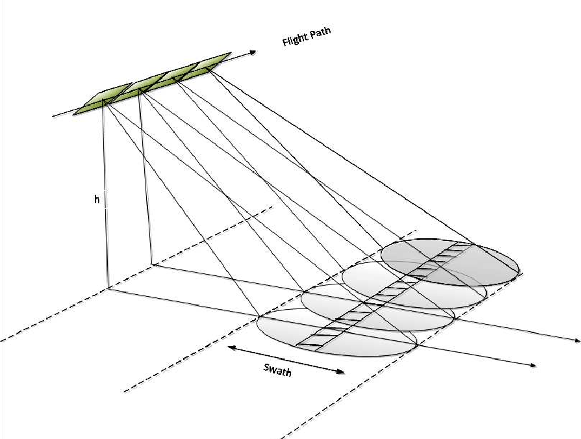
\includegraphics[height=5cm]{sar (2).png}	
	\caption{Working of SAR}
	\label{fig:1}			
\end{figure}




\section{Analysis}
\subsection{SAR Data}\label{sec:sar_data}
SAR is a coherent imaging method which returns two components, the intensity and the phase. \\
The visible image formed after SAR image processing has occurred is the intensity component of the SAR data.
Upon transmission, the radio waves in the SAR beam are coherent (as in, they are aligned in space and time). These radio waves are said to be "in phase". 
The radio waves shift and no longer stay in phase with each other when they interact with scatterers on the surface of the terrain. The amount of shift "out of phase" is measured and is represented by the phase component of the SAR data. These phase components reveal the geometry and composition of the landscape.
% The intensity component of SAR data is the part that looks like an image after SAR image formation processing has occurred. The radio waves in the SAR beam are aligned in space and time (coherent) upon transmission, or in other words they are “in phase.” 
% The phase component of SAR data measures how much the radio waves have shifted “out of phase” after they interact with the scatterers on the surface. These phase components are useful, because phase differences between different channels or different collects can reveal information about the geometry and composition of the scene.\\
%  Single Look Complex\\
% SAR data can be delivered as Single Look Complex (SLC) data where the intensity and phase components are represented as complex numbers for each pixel. Intensity and phase values can be subsequently computed from the complex numbers. Intensity and phase can be viewed as images, as seen in Figure 1, though only the intensity component is recognizable as an image. Additionally, SLC data is in the radar-image (slant) plane projection, so its pixels do not correspond to geo-coordinates.\\
% Ground Range Detected\\
% SAR data can also be delivered as Ground Range Detected (GRD) data, in which processing has been done to project the image onto the ground plane with geo-coordinates such as latitude and longitude, creating a terrain map.\\
% Speckle Reduction\\
% There are various methods to achieve speckle reduction and make a SAR image easier to interpret and analyse. Multi-looking is the process of splitting the radar beam into several narrower sub-beams. Each of these sub-beams is a “look” and is subject to speckle. However all the “looks” can be averaged and the amount of speckle in the final averaged image will be reduced. Another method of speckle reduction is spatial filtering, in which a “moving window” technique is used to calculate a weighted average of a group of pixels and replace the window’s center pixel with that value. This technique produces a smoothing effect in which the amount of speckle is reduced.

\section{Citations}\label{sec:citations}
All sources should be cited, the \verb|\autocite| command from Bib\LaTeX\ is the best to use. For example, the command \verb|\autocite{BrandonD.G2008Mcom}| is typeset as \autocite{BrandonD.G2008Mcom}. Some other commands can be useful, these can be investigated in section~3.9 of the \href{http://mirror.ox.ac.uk/sites/ctan.org/macros/latex/contrib/biblatex/doc/biblatex.pdf}{Bib\LaTeX\ user manual}.


\printbibliography			%inserts the bibliography, remember to specify your bib file in the preamble!
\end{document}